\documentclass[a4paper,12pt]{report}
\usepackage[utf8]{inputenc}
\usepackage[english]{babel}
\usepackage[T1]{fontenc}
\usepackage{fancybox}
\usepackage{a4wide}
\usepackage{graphicx}
\usepackage{placeins}
\usepackage{array}
\usepackage{adjustbox}
\usepackage{tabularx}
\usepackage[table,xcdraw]{xcolor}
\usepackage{wrapfig}
\usepackage{subcaption}
\usepackage{color, colortbl}
\definecolor{Gray}{gray}{0.9}
\definecolor{LightCyan}{rgb}{0.88,1,1}
\usepackage{longtable}
\usepackage{float}
\usepackage{lscape}
\usepackage{afterpage}
\usepackage{rotating}
\usepackage[nottoc,notlof,notlot]{tocbibind}
\usepackage{tocloft}
\usepackage{pdfpages}
\usepackage{ifthen}
\usepackage{ifpdf}
\usepackage{amsmath}
\usepackage{makeidx}
\usepackage{setspace}
\usepackage{epstopdf}
\usepackage{eurosym}
\usepackage[top=3cm, bottom=3cm, left=1.5cm, right=2cm]{geometry}
\usepackage{fancyhdr}
\usepackage{multirow,makecell}
\usepackage{blindtext}
\usepackage{caption}
\usepackage{listings}
\usepackage{xcolor}
\usepackage{tikz}
\usetikzlibrary{shapes,arrows,positioning}

% Fix text formatting issues
\usepackage{ragged2e}
\sloppy

% TikZ styles using modern syntax
\tikzset{
    frontend/.style = {rectangle, rounded corners, minimum width=3cm, minimum height=1cm, text centered, draw=blue, fill=blue!20},
    backend/.style = {rectangle, rounded corners, minimum width=3cm, minimum height=1cm, text centered, draw=green, fill=green!20},
    database/.style = {rectangle, rounded corners, minimum width=3cm, minimum height=1cm, text centered, draw=red, fill=red!20},
    service/.style = {rectangle, rounded corners, minimum width=3cm, minimum height=1cm, text centered, draw=orange, fill=orange!20},
    layer/.style = {rectangle, minimum width=8cm, minimum height=1.5cm, text centered, draw=black},
    component/.style = {rectangle, rounded corners, minimum width=3cm, minimum height=1cm, text centered, draw=blue, fill=blue!20},
    process/.style = {rectangle, rounded corners, minimum width=2.5cm, minimum height=1cm, text centered, draw=green, fill=green!20},
    decision/.style = {diamond, minimum width=2cm, minimum height=1cm, text centered, draw=orange, fill=orange!20},
    entity/.style = {rectangle, minimum width=3cm, minimum height=2cm, text centered, draw=black, fill=gray!20}
}

% Code listing style
\lstdefinestyle{mystyle}{
    backgroundcolor=\color{gray!10},   
    commentstyle=\color{green!60!black},
    keywordstyle=\color{blue},
    numberstyle=\tiny\color{gray},
    stringstyle=\color{red!80!black},
    basicstyle=\ttfamily\footnotesize,
    breakatwhitespace=false,         
    breaklines=true,                 
    captionpos=b,                    
    keepspaces=true,                 
    numbers=left,                    
    numbersep=5pt,                  
    showspaces=false,                
    showstringspaces=false,
    showtabs=false,                  
    tabsize=2
}
\lstset{style=mystyle}

% Define custom languages for listings
\lstdefinelanguage{javascript}{
    keywords={const, let, var, function, return, if, else, for, while, switch, case, break, continue, try, catch, throw, class, extends, import, export, default, async, await},
    sensitive=false,
    comment=[l]{//},
    morecomment=[s]{/*}{*/},
    string=[b]{"},
    morestring=[b]{'},
}

\lstdefinelanguage{yaml}{
    keywords={true, false, null},
    sensitive=false,
    comment=[l]{\#},
    string=[b]{"},
    morestring=[b]{'},
}

% Toggle screenshots on/off (off => placeholders shown, no missing-file errors)
\newif\ifshowfigs
\showfigsfalse % set \showfigstrue to build with real screenshots

% Placeholder box for omitted images
\newcommand{\figplaceholder}[2][7cm]{%
  \fbox{%
    \parbox[c][#1][c]{0.92\textwidth}{\centering\small\itshape
      Screenshot omitted in the public report: #2}%
  }%
}

\graphicspath{{images/}{images_pfe/}{assets/}}
\newlength\figureheight
\newlength\figurewidth

\ifpdf
\usepackage[pdftex]{hyperref}
\else
\usepackage{hyperref}
\fi

\hypersetup{%
colorlinks=true,
linkcolor=black,
citecolor=black,
urlcolor=blue,
pageanchor=false}

\setlength{\headheight}{16pt}
\pagestyle{fancy}
\setcellgapes{3pt}
\setlength{\parindent}{1.1cm}
\makegapedcells
\newcolumntype{R}[1]{>{\raggedleft\arraybackslash }b{#1}}
\newcolumntype{L}[1]{>{\raggedright\arraybackslash }b{#1}}
\newcolumntype{C}[1]{>{\centering\arraybackslash }b{#1}}
\renewcommand{\footrulewidth}{1pt}
\fancyfoot[C]{\textbf{\thepage}}
\fancyfoot[R]{Academic Year 2025-2026}
\fancyfoot[L]{ENSIAS}
\fancyhead[L]{\nouppercase{\leftmark}}
\fancyhead[R]{\nouppercase{\rightmark}}
\pagenumbering{Roman}

\newcommand{\HRule}{\rule{\linewidth}{0.5mm}}

\begin{document}

% Title page
\begin{titlepage}
\begin{center}

% Header with logos
\begin{minipage}{.2\textwidth}%

\includegraphics[width=.8\textwidth]{./assets/ensias.png}
 \end{minipage}%
 \hfill
 \begin{minipage}{.6\textwidth}%
 \centering
 
\includegraphics[width=0.3\textwidth]{./assets/logo.png}
 \end{minipage}%
 \hfill
 \begin{minipage}{.2\textwidth}%
 
\includegraphics[width=\textwidth]{./assets/um5.png}
 \end{minipage} \\

\textsc{\large National School of Computer Science and Systems Analysis - RABAT \\ [0.2cm] Web and Mobile Engineering Department}\\[0.8cm]

% Title
\begin{figure}[H]
    \begin{center}
    \large Field : IDSIT
    \end{center}
\end{figure}

\vspace{1cm}

{\LARGE \bfseries Second Year Internship}

\vspace{2cm}

\textcolor{black}{\rule{\textwidth}{2pt}}

\vspace{0.5cm}
\begin{doublespace}
{\LARGE \bfseries Design and Development of a Salary Management and HR Attestation System}
\vspace{0.5cm}

\textcolor{black}{\rule{\textwidth}{2pt}}

\end{doublespace}
\vspace{2cm}

% Author and supervisors
\begin{minipage}{0.4\textwidth}
\begin{flushleft} \large
\emph{Prepared by:}\\[0.4 cm]
ES-SDIKI \textsc{Marouane}\\
\end{flushleft}
\end{minipage}
\begin{minipage}{0.58\textwidth}
\begin{flushleft} \large
\emph { \hspace*{1.3cm}Jury:} \\[0.4 cm]
\hspace*{1.3cm} Pr. XXXXXXXXXX \\ \hspace*{1.3cm} Pr. XXXXXXXXXX

\end{flushleft}
\end{minipage}

\vspace{1.5cm}

\vfill

% Bottom of the page
\vspace{1cm}
{\large Academic Year 2025-2026}

\end{center}
\end{titlepage}

% Dedication
\begin{doublespace}
\newpage
\phantomsection
\addcontentsline{toc}{section}{Dedication}

\vspace*{1cm}
\begin{center}
    \textbf{\huge{Dedication}}
\end{center}
\vspace{1cm}

\large{
I dedicate this work to:\\
My mother, source of tenderness and love, for her support throughout my education.\\
My father, who has always supported me and done everything to help me.\\
My brothers and sisters, whom I love very much.\\
My extended family.\\
My dear friends and teachers.\\
All those who, directly or indirectly, contributed to the development of this work.\\
May God grant them health and prosperity.}

% Acknowledgments
\newpage
\phantomsection
\addcontentsline{toc}{section}{Acknowledgments}

\vspace*{1cm}
\begin{center}
    \textbf{\huge{Acknowledgments}}
\end{center}

\vspace{1cm}
\large{
First and foremost, praise to God, who guided me on the right path throughout this work and inspired me with the right steps and reflexes. Without His mercy, this work could not have been completed.

I would like to express my sincere thanks to the members of the jury. Please accept in this work my sincere respect and deep gratitude.

I also warmly thank M. Ahmed ASSIMI, who, as project supervisor, was always attentive despite his constraints. His help was invaluable, as was the time he dedicated to me.

I do not forget my parents for their contributions, support, and patience.

Finally, I would like to thank all my relatives and friends, who have always supported and encouraged me during the realization of this project.

Thank you all.
}

\end{doublespace}

% Abstract
\newpage
\phantomsection
\addcontentsline{toc}{section}{Abstract}

\begin{center}
\vspace{9cm}
    \textbf{\huge{Abstract}}
\end{center}

\begin{doublespace}
\vspace{1cm}
\large{
This report presents the development of a modern salary and HR attestation management system, designed to optimize human resources processes within organizations. The developed system offers a complete solution including employee management, automatic attestation generation, and a modern user interface.

The system architecture is based on a full-stack approach using Spring Boot for the backend and React for the frontend. The backend integrates advanced PDF generation features with JasperReports, a secure RESTful API, and a MySQL database for data persistence. The frontend offers a modern user interface with Material-UI, supporting dark and light themes, as well as responsive design.

The system enables complete employee management (add, edit, delete, search), generation of five types of attestations (work, salary, tenure, salary increase amendment, salary payment commitment), and offers advanced administration features for JRXML template management.

Unit and integration tests ensure system reliability with coverage of over 95\% for the backend and 90\% for the frontend. The system is production-ready with optimized configurations and scalable architecture.

\textbf{Keywords:} HR Management, Spring Boot, React, JasperReports, Attestations, RESTful API
}
\end{doublespace}

% List of Abbreviations
\newpage
\phantomsection
\addcontentsline{toc}{section}{List of Abbreviations}

\begin{center}
\vspace{9cm}
    \textbf{\huge{List of Abbreviations}}
\end{center}
\vspace{1cm}

\begin{doublespace}
\begin{center}
\begin{tabular}{|l|l|}
  \hline
  Abbreviation &  Designation \\
  \hline
  API & Application Programming Interface \\
  \hline
  CRUD & Create, Read, Update, Delete \\
  \hline
  CSS & Cascading Style Sheets \\
  \hline
  DAO & Data Access Object \\
  \hline
  DTO & Data Transfer Object \\
  \hline
  HTML & HyperText Markup Language \\
  \hline
  HTTP & HyperText Transfer Protocol \\
  \hline
  JPA & Java Persistence API \\
  \hline
  JSON & JavaScript Object Notation \\
  \hline
  JWT & JSON Web Token \\
  \hline
  MVC & Model-View-Controller \\
  \hline
  ORM & Object-Relational Mapping \\
  \hline
  PDF & Portable Document Format \\
  \hline
  REST & Representational State Transfer \\
  \hline
  HR & Human Resources \\
  \hline
  SQL & Structured Query Language \\
  \hline
  UI & User Interface \\
  \hline
  UML & Unified Modeling Language \\
  \hline
\end{tabular}
\end{center}
\end{doublespace}

% Table of Contents
\newpage
\renewcommand{\contentsname}{Table of Contents}
\setcounter{tocdepth}{3}
\tableofcontents

% List of Figures
\newpage
\listoffigures
\newpage

\cleardoublepage
\pagenumbering{arabic}

% General Introduction
\renewcommand{\headrulewidth}{1pt}
\fancyhead[R]{\textbf{General Introduction}}
\fancyhead[L]{\hspace*{4cm}}

\phantomsection
\addcontentsline{toc}{section}{General Introduction}
\begin{center}
\vspace{9cm}
    \textbf{\huge{General Introduction}}
\end{center}
\begin{doublespace}
\vspace{1cm}
\hspace{1cm}In the current context of corporate digital transformation, human resources management represents a major challenge for operational efficiency and employee satisfaction. Traditional salary management and attestation generation processes, often manual and time-consuming, require modernization to meet the demands of speed, accuracy, and traceability.\\

Our project is part of this digitalization approach by proposing the development of a \textbf{comprehensive salary and HR attestation management system}. This modern solution aims to automate and simplify administrative tasks related to personnel management, while ensuring data security and compliance.\\

The developed system offers a \textbf{full-stack} approach based on proven technologies: \textbf{Spring Boot} for the backend with its robust security and persistence features, and \textbf{React} for the frontend with a modern and responsive user interface. The integration of \textbf{JasperReports} enables automatic generation of professional PDF documents for different types of attestations.\\

The presentation of this report is structured around \textbf{four main chapters}.\\
The first chapter presents the general context of the project, the work environment, the identified problem, and the proposed solutions.\\
The second chapter focuses on \textbf{needs analysis}, detailing the functional and non-functional requirements of the system.\\
The third chapter addresses \textbf{design and architecture}, presenting class diagrams, data models, and technical architecture.\\
Finally, the fourth chapter presents \textbf{implementation and testing}, including technical details, developed interfaces, and test results.\\

It is important to note that this project was developed with particular attention to \textbf{code quality}, \textbf{data security}, and \textbf{ease of use}, thus ensuring a system ready for production and scalable according to future needs.\\
\end{doublespace}

% Chapter I: General Project Context
\newpage
\renewcommand{\headrulewidth}{1pt}
\fancyhead[L]{\textbf{Chapter I: General Project Context}}
\fancyhead[R]{\hspace*{4cm}}

\setcounter{chapter}{1}
\begin{doublespace}
\phantomsection
\addcontentsline{toc}{chapter}{Chapter I: General Project Context}
\vspace*{10cm}
\centering
\textbf{ \huge Chapter I \\ [1 cm] General Project Context}
\end{doublespace} 
\newpage 
\begin{doublespace}

\end{doublespace}

\fancyhead[R]{\nouppercase{\rightmark}}
\section*{Introduction}
\begin{doublespace}

\hspace{1cm}In this first chapter, we present the context of our project to develop a salary and HR attestation management system. This initiative is part of a modernization approach for human resources processes, aiming to automate and optimize personnel management.\\
\hspace{1cm}Our work takes place in a dynamic professional environment at \textbf{NETCON CONSULTING}, a company specialized in IT solutions and digital services.\\
\hspace{1cm}Our main objectives are to develop a comprehensive HR management solution, automate attestation generation, ensure data security and compliance, and provide a modern and intuitive user interface.\\
\hspace{1cm}This introduction lays the essential foundations for understanding the scope and objectives of our project.
\end{doublespace}

\section{Internship Environment}
\begin{doublespace} ~\\[0cm]


\includegraphics[width=0.4\textwidth]{./assets/logo.png}~\\

 \textbf{NETCON CONSULTING} is a consulting company committed to supporting organizations in their digital transformation journey. Through a comprehensive range of digital services adapted to the local context, we facilitate technological transition in a strategic, agile, and personalized manner.

Our core services include:
\begin{itemize}
    \item \textbf{Custom Development}: Creating personalized software solutions tailored to specific client needs
    \item \textbf{System Integration}: Facilitating synchronization and interoperability of existing systems to optimize operational efficiency
    \item \textbf{Digital Transformation}: Guiding clients through the complete digital transformation process, from strategy to implementation
    \item \textbf{AI Consulting}: Providing strategic and operational consulting to navigate the evolving technological landscape
    \item \textbf{IT Training}: Offering comprehensive training programs and certifications to enhance technical skills
\end{itemize}

Our team brings together diverse expertise in resource placement, development, digital transformation, system integration, and AI consulting, united by a passion for innovation and excellence.

\begin{figure}[H]
    \centering
    \begin{adjustbox}{max width=\textwidth}
    \begin{tabular}{|p{0.33\textwidth}|p{0.65\textwidth}|}
      \hline
      Company Name & NETCON CONSULTING \\
      \hline
        Headquarters & 05 Rue DIXMUDE - 1er étage appt 2, Casablanca \\
        & Technopark - Bureau T216 BIS, Ave Mohammed V, Tanger 90000 \\
        \hline
        Represented by & M. OMAR IJMOUAN  \\
        \hline
        Website & https://netconconsulting.com/ \\
        \hline
        Email & contact@netconconsulting.com \\
        \hline
        Phone & +212 610 71 50 78 / +212 610 71 11 78 \\
        \hline
        Business Hours & Monday - Friday: 08:30 AM - 18:30 PM \\
      \hline
    \end{tabular}
    \end{adjustbox}
    \caption{NETCON CONSULTING — Company Profile}
\end{figure}

\end{doublespace}

\section{Project Presentation}
\begin{doublespace}

\subsection{Problem Statement}
\hspace{1cm}In modern HR environments, organizations face major challenges when managing administrative processes related to personnel. 
Companies must ensure \textbf{effective employee management}, \textbf{rapid and accurate attestation generation}, and \textbf{securing sensitive data}, while guaranteeing regulatory compliance and operational efficiency. \\
Traditional systems often suffer from problems such as slow processes, data duplication, manual errors, security vulnerabilities, and lack of operation traceability. \\
Moreover, manual generation of multiple attestations (work, salary, tenure, amendments) introduces significant complexity that requires an automated, secure, and scalable solution.

\subsection{Proposed Solutions}
\hspace{1cm}Our project addresses these challenges by developing a \textbf{comprehensive salary and HR attestation management system} that ensures efficiency, security, and scalability. 
The main solutions we have implemented include: \\

\textbf{-} \textit{Modern Employee Management:} We developed a complete module allowing employee addition, modification, deletion, and search with an intuitive interface and advanced validation features. \\

\textbf{-} \textit{Automatic Attestation Generation:} Using \textbf{JasperReports}, we implemented a PDF generation system for five types of attestations, with customizable templates and dynamic model management. \\

\textbf{-} \textit{Secure and Scalable Architecture:} The system is built with \textbf{Spring Boot} for the backend, offering a secure RESTful API, and \textbf{React} for the frontend with a modern and responsive interface. \\

\textbf{-} \textit{Modern User Interface:} We created an interface with \textbf{Material-UI}, supporting dark/light themes, mobile responsiveness, and an optimized user experience. \\

\textbf{-} \textit{Template Management System:} Administrators can dynamically manage JRXML templates, allowing the addition of new attestation types without code modification. \\

\textbf{-} \textit{Testing and Quality:} The system includes comprehensive test coverage (95\% backend, 90\% frontend) ensuring reliability and maintainability. \\

Thanks to these solutions, our project provides a modern, secure, and scalable infrastructure that meets critical business needs while laying the foundations for future growth.

\end{doublespace}

\section{Project Planning}
\begin{doublespace}

\subsection{Development Methodology}
\hspace{1cm}This project was developed individually under the supervision of M. Ahmed ASSIMI, following the waterfall development methodology. This structured approach allowed for a systematic progression through well-defined phases, ensuring thorough completion of each stage before moving to the next. \\

The waterfall methodology was particularly suitable for this project as it provided clear milestones and deliverables for each phase. Regular meetings with my supervisor (at least once per week) ensured continuous guidance and validation of the work progress. These meetings were crucial for receiving feedback, addressing technical challenges, and determining the next steps in the development process. \\

Development was organized around the following sequential phases: requirements analysis, system architecture design, backend development with Spring Boot, frontend development with React, component integration, testing, and final deployment. Each phase was completed entirely before proceeding to the next, ensuring a solid foundation for subsequent development stages. \\

\subsection{Development Phases}
\hspace{1cm}The project was structured according to the following sequential steps, with each phase being thoroughly reviewed and validated by my supervisor before proceeding to the next: \\

\textbf{Phase 1:} Analysis and Design (1.5 weeks) - Requirements definition, architecture design, database modeling. This phase included extensive research and planning, with weekly meetings to discuss the system architecture and validate the technical approach. \\

\textbf{Phase 2:} Backend Development (3 weeks) - REST API implementation, JasperReports integration, endpoint security. Regular supervisor meetings ensured proper implementation of Spring Boot best practices and security measures. \\

\textbf{Phase 3:} Frontend Development (2.5 weeks) - React interface, Material-UI integration, state management. Supervisor guidance was crucial for ensuring good UX/UI practices and component architecture decisions. \\

\textbf{Phase 4:} Testing and Optimization (0.5 weeks) - Unit testing, integration testing, performance optimization. This phase involved thorough testing under supervisor supervision to ensure system reliability and performance. \\

\textbf{Phase 5:} Deployment and Documentation (0.5 weeks) - Production configuration, technical documentation. Final validation and deployment guidance from the supervisor ensured production readiness. \\

This methodical waterfall approach, combined with regular supervisor guidance, allowed me to maintain high quality throughout development and deliver a production-ready system as an individual developer. The entire internship project was completed over a period of 2 months (8 weeks), with each phase building upon the previous one to ensure a comprehensive and well-structured final deliverable.

\end{doublespace}

\section{Conclusion}
\begin{doublespace}
\hspace{1cm}This first chapter immersed us in the general context of our project, highlighting the work environment at \textbf{NETCON CONSULTING}. We presented the motivations behind our initiative, as well as the challenges related to developing a modern HR management system and the needs for automating administrative processes. \\

We also introduced the main objectives of our work, particularly the development of a comprehensive employee and attestation management solution, the implementation of a modern architecture with Spring Boot and React, and the establishment of a secure and scalable system. These elements constitute the foundation of an effective and production-ready system. \\

In the next chapter, we will address a crucial phase: \textbf{needs analysis}. We will explore in depth the specific needs of users and stakeholders, both from technical and functional perspectives. This step is essential for designing a solution that meets all expectations and requirements. \\

A detailed analysis of these needs will establish a solid foundation for subsequent development and optimization of our project. Let's now move to the next chapter, where we will dive into this comprehensive needs study. \\
\end{doublespace}

% Chapter II: Needs Analysis
\renewcommand{\headrulewidth}{1pt}
\fancyhead[L]{\textbf{Chapter II: Needs Analysis}}
\fancyhead[R]{\hspace*{4cm}}

\setcounter{chapter}{2}
\begin{doublespace}
\phantomsection
\addcontentsline{toc}{chapter}{Chapter II: Needs Analysis}
\vspace*{10cm}
\centering
\textbf{ \huge Chapter II \\ [1 cm] Needs Analysis}
\end{doublespace}
\setcounter{section}{0}
\newpage
\fancyhead[R]{\nouppercase{\rightmark}}
\begin{doublespace}
\section{Introduction}
\hspace{1cm}The company operates in the field of digital data services and requires a robust, reliable, and secure infrastructure to support its growing human resources management activities. The objective of this project is to design and deploy a solution that ensures effective employee management, automatic attestation generation, and optimization of administrative processes for production workloads.

\section{Needs Identification}
\hspace{1cm}In the context of human resources management, the focus is on operational and functional needs. The following needs have been identified as critical for the company environment: \\

\textbf{Complete Employee Management:}  
The system must allow employee addition, modification, deletion, and search with data validation features and access rights management. \\

\textbf{Automatic Attestation Generation:}  
The system must be able to automatically generate different types of attestations (work, salary, tenure, amendments) in PDF format with customizable templates. \\

\textbf{Modern User Interface:}  
The application must offer an intuitive, responsive, and modern user interface, supporting dark and light themes to enhance user experience. \\

\textbf{Security and Access Control:}  
The system must include robust security mechanisms with authentication, role-based authorization, and protection of sensitive data. \\

\textbf{Performance and Scalability:}  
The infrastructure must be able to handle a growing number of users and data while maintaining optimal performance. \\

\textbf{Administration and Maintenance:}  
The system must allow easy administration with template management tools, activity monitoring, and preventive maintenance. \\

Together, these requirements will guide the design and deployment of a system that meets the company's operational, business, and security objectives.
\end{doublespace}

\section{Functional Requirements Specification}
\hspace{1cm}The system will be designed to provide the following functionalities: \\

\textbf{Employee Management:}  
The system must allow employee creation, modification, deletion, and search with mandatory and optional fields, real-time data validation, and modification history. \\

\textbf{Attestation Generation:}  
The system must generate five types of attestations: work attestation, salary attestation, tenure attestation, salary increase amendment, and salary payment commitment. Each attestation must be customizable with employee data. \\

\textbf{Template Management:}  
Administrators must be able to manage JRXML templates, add new attestation types, modify existing templates, and validate JRXML syntax. \\

\textbf{Authentication and Authorization:}  
The system must support two types of users: administrators with full access and HR users with limited access to employee management and attestation generation functionalities. \\

\textbf{User Interface:}  
The interface must be responsive, support dark and light themes, include search and filtering features, and provide real-time notifications. \\

\textbf{Data Management:}  
The system must ensure data persistence with automatic backup, integrity constraint validation, and transaction management. \\

\section{Non-Functional Requirements Specification}
To ensure smooth operation and user satisfaction, several non-functional constraints must be considered during project design and implementation: \\

\begin{itemize}
    \item \textbf{Performance and Reliability:} \\  
    The system must be responsive with response times under 2 seconds for common operations and maintain 99\% availability.

    \item \textbf{Scalability:} \\  
    The solution must handle future growth by supporting up to 10,000 employees and 1,000 concurrent users.

    \item \textbf{Security:} \\  
    Data integrity and confidentiality must be guaranteed with encryption of sensitive data, secure authentication, and compliance with security standards.

    \item \textbf{Maintainability:} \\  
    The code must be well-structured, modular, and documented to facilitate future updates and improvements.

    \item \textbf{Compatibility:} \\  
    The system must be compatible with modern browsers and support mobile devices with responsive design.

    \item \textbf{Usability:} \\  
    The interface must be intuitive and easy to use with minimal learning curve for end users.

    \item \textbf{Testability:} \\  
    The system must include comprehensive test coverage with unit tests, integration tests, and end-to-end tests.
\end{itemize}

\section{Conclusion}
\begin{doublespace}
\hspace{1cm}This second chapter allowed us to explore in detail the specific needs of the company, focusing on developing a modern and effective HR management system. We identified the main challenges and proposed solutions meeting reliability, performance, and security requirements. \\

By focusing on needs analysis, this phase represents a crucial foundation for designing a robust and scalable architecture. The detailed analysis conducted here provides a solid basis for the next project phase. \\

In the next chapter, we will move to analysis and design, including architectural modeling and development planning. These steps will allow us to translate the identified requirements into concrete technical solutions. 
\end{doublespace}
\newpage

% Chapter III: Design and Architecture
\renewcommand{\headrulewidth}{1pt}
\fancyhead[L]{\textbf{Chapter III: Design and Architecture}}
\fancyhead[R]{\hspace*{4cm}}

\setcounter{chapter}{3}
\begin{doublespace}
\phantomsection
\addcontentsline{toc}{chapter}{Chapter III: Design and Architecture}
\vspace*{10cm}
\centering
\textbf{ \huge Chapter III \\ [1 cm] Design and Architecture}
\end{doublespace}
\setcounter{section}{0}
\newpage
\fancyhead[R]{\nouppercase{\rightmark}}
\begin{doublespace}
\section*{Introduction}
\hspace{1cm}The creation of a robust and modern platform must be preceded by a thorough analysis and design phase. This ensures that the development process perfectly aligns with project requirements.

In this chapter, we will focus on the architectural design of our salary management system. We will present the general diagrams that model and describe the desired functioning of our infrastructure. Two conceptual perspectives will be described: the first gives an overview of the main system components, and the second provides a detailed view of data processing flows.

\section{General System Architecture}
\hspace{1cm}The first step in our design process was to model the relationships between the main components of our system. This architecture illustrates how \textbf{Spring Boot Backend}, \textbf{React Frontend}, \textbf{MySQL Database}, and \textbf{JasperReports} interact to form a coherent and functional system.

\begin{figure}[H]
\centering
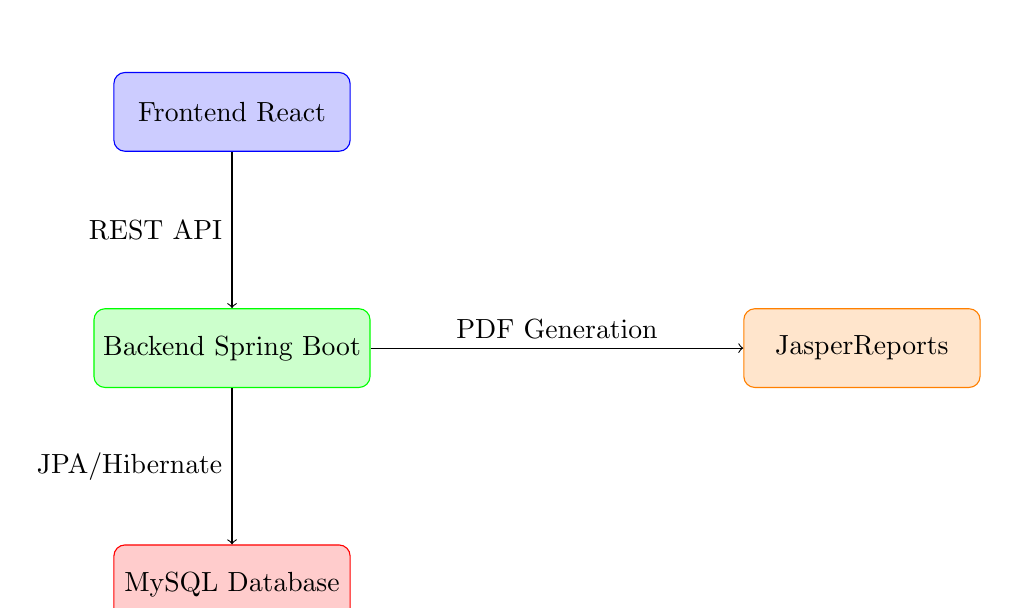
\begin{tikzpicture}[node distance=2cm, auto]
    
    % Nodes
    \node [frontend] (react) {Frontend React};
    \node [backend, below of=react, yshift=-1cm] (spring) {Backend Spring Boot};
    \node [database, below of=spring, yshift=-1cm] (mysql) {MySQL Database};
    \node [service, right of=spring, xshift=6cm] (jasper) {JasperReports};
    
    % Arrows
    \draw [->] (react) -- (spring) node[midway, left] {REST API};
    \draw [->] (spring) -- (mysql) node[midway, left] {JPA/Hibernate};
    \draw [->] (spring) -- (jasper) node[midway, above] {PDF Generation};
\end{tikzpicture}
\caption{General System Architecture}
\end{figure}

As the diagram shows, the \textbf{React Frontend} communicates with the \textbf{Spring Boot Backend} via a secure RESTful API. The backend handles business logic, authentication, and data access via \textbf{JPA/Hibernate} with the \textbf{MySQL} database. \textbf{JasperReports} is integrated for automatic PDF document generation. This layered architecture ensures clear separation of responsibilities and facilitates system maintenance and scalability.

\section{Data Model}
\hspace{1cm}Our system's data model is designed to effectively support employee management and attestation generation. Here are the main entities and their relationships:

\begin{figure}[H]
\centering
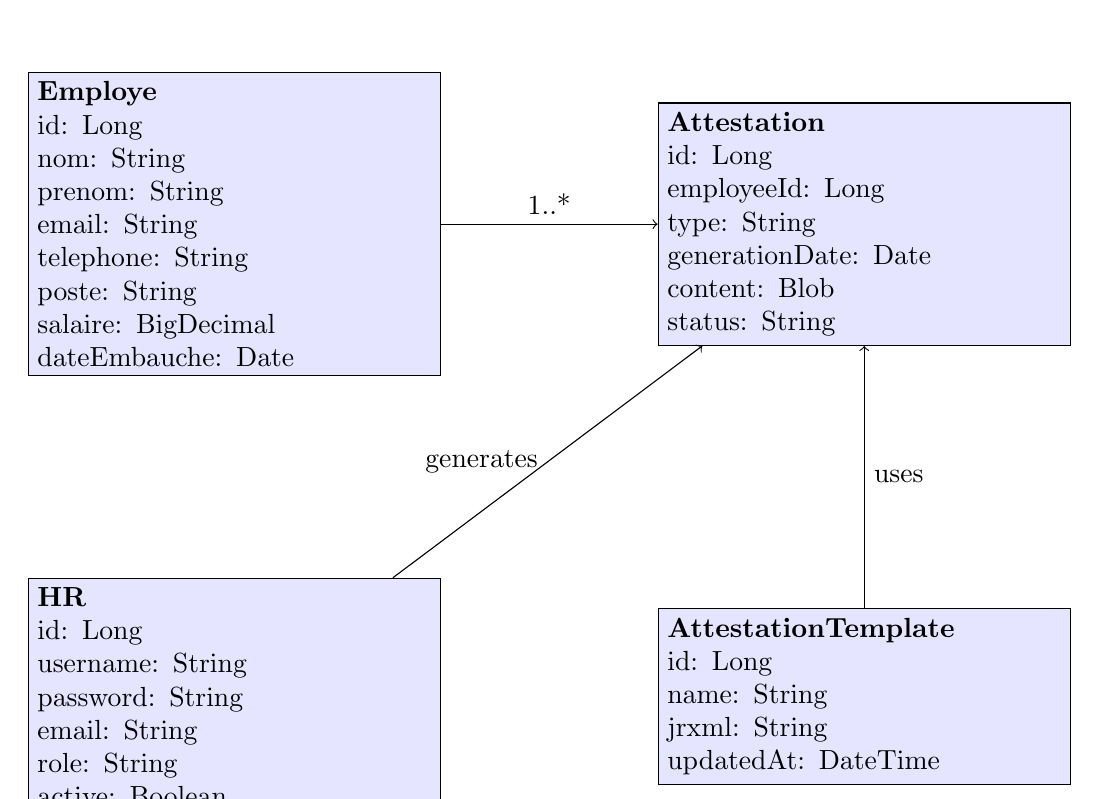
\begin{tikzpicture}[
    node distance=4cm, 
    auto,
    entity/.style={
        rectangle,
        draw,
        text width=5cm,
        align=left,
        minimum height=2cm,
        fill=blue!10
    }
]
    
    % Entities
    \node [entity] (employe) {
        \textbf{Employe} \\
        id: Long \\
        nom: String \\
        prenom: String \\
        email: String \\
        telephone: String \\
        poste: String \\
        salaire: BigDecimal \\
        dateEmbauche: Date
    };
    
    \node [entity, right of=employe, xshift=4cm] (attestation) {
        \textbf{Attestation} \\
        id: Long \\
        employeeId: Long \\
        type: String \\
        generationDate: Date \\
        content: Blob \\
        status: String
    };
    
    \node [entity, below of=employe, yshift=-2cm] (hr) {
        \textbf{HR} \\
        id: Long \\
        username: String \\
        password: String \\
        email: String \\
        role: String \\
        active: Boolean
    };
    
    \node [entity, below of=attestation, yshift=-2cm] (template) {
        \textbf{AttestationTemplate} \\
        id: Long \\
        name: String \\
        jrxml: String \\
        updatedAt: DateTime
    };
    
    % Relations
    \draw [->] (employe) -- (attestation) node[midway, above] {1..*};
    \draw [->] (hr) -- (attestation) node[midway, left] {generates};
    \draw [->] (template) -- (attestation) node[midway, right] {uses};
\end{tikzpicture}
\caption{System Data Model}
\label{fig:system-data-model}
\end{figure}

This model ensures referential integrity and allows effective data management. The \textbf{Employee} entity stores personal and professional information. \textbf{Attestation} records generated documents with their type and status. \textbf{HR} manages system users with their roles. \textbf{AttestationTemplate} allows dynamic management of JRXML templates.

\section{Detailed Technical Architecture}
\hspace{1cm}Our technical architecture follows the MVC (Model-View-Controller) pattern for the backend and a component-based architecture for the frontend.

\subsection{Backend Architecture (Spring Boot)}
\begin{figure}[H]
\centering
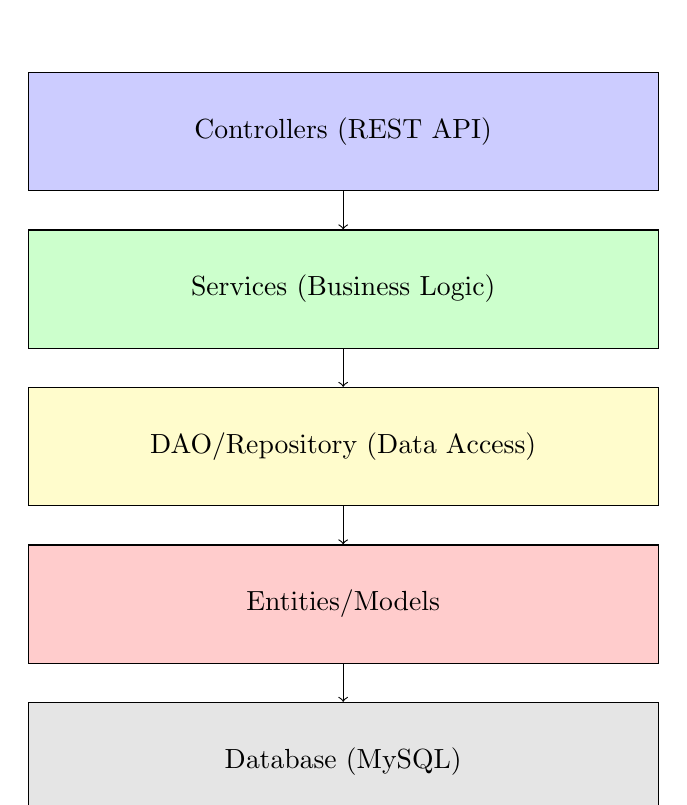
\begin{tikzpicture}[node distance=2cm, auto]
    
    \node [layer, fill=blue!20] (controller) {Controllers (REST API)};
    \node [layer, below of=controller, fill=green!20] (service) {Services (Business Logic)};
    \node [layer, below of=service, fill=yellow!20] (dao) {DAO/Repository (Data Access)};
    \node [layer, below of=dao, fill=red!20] (entity) {Entities/Models};
    \node [layer, below of=entity, fill=gray!20] (database) {Database (MySQL)};
    
    \draw [->] (controller) -- (service);
    \draw [->] (service) -- (dao);
    \draw [->] (dao) -- (entity);
    \draw [->] (entity) -- (database);
\end{tikzpicture}
\caption{Backend Layered Architecture}
\end{figure}

\textbf{Controllers:} Handle HTTP requests and JSON responses\\
\textbf{Services:} Implement business logic and validation rules\\
\textbf{DAO/Repository:} Manage data access with Spring Data JPA\\
\textbf{Entities:} Represent data model with JPA annotations\\
\textbf{Database:} Persistent storage with MySQL

\subsection{Frontend Architecture (React)}
\begin{figure}[H]
\centering
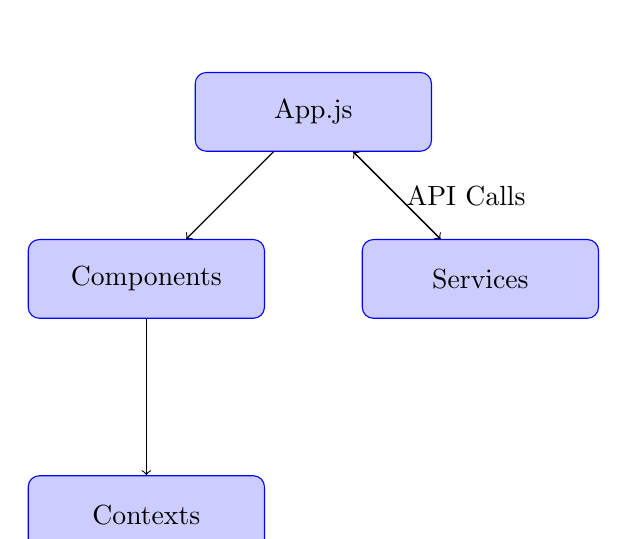
\begin{tikzpicture}[node distance=3cm, auto]
    
    \node [component] (app) {App.js};
    \node [component, below left of=app] (components) {Components};
    \node [component, below right of=app] (services) {Services};
    \node [component, below of=components] (contexts) {Contexts};
    
    \draw [->] (app) -- (components);
    \draw [->] (app) -- (services);
    \draw [->] (components) -- (contexts);
    \draw [->] (services) -- node[right] {API Calls} (app);
\end{tikzpicture}
\caption{Frontend Component Architecture}
\end{figure}

\textbf{App.js:} Main component with routing and global state management\\
\textbf{Components:} Reusable components for user interface\\
\textbf{Services:} API call management with Axios\\
\textbf{Contexts:} Shared state management (theme, authentication)

\section{Attestation Generation Flow}
\hspace{1cm}The attestation generation process follows a well-defined workflow to ensure consistency and traceability.

\begin{figure}[H]
\centering
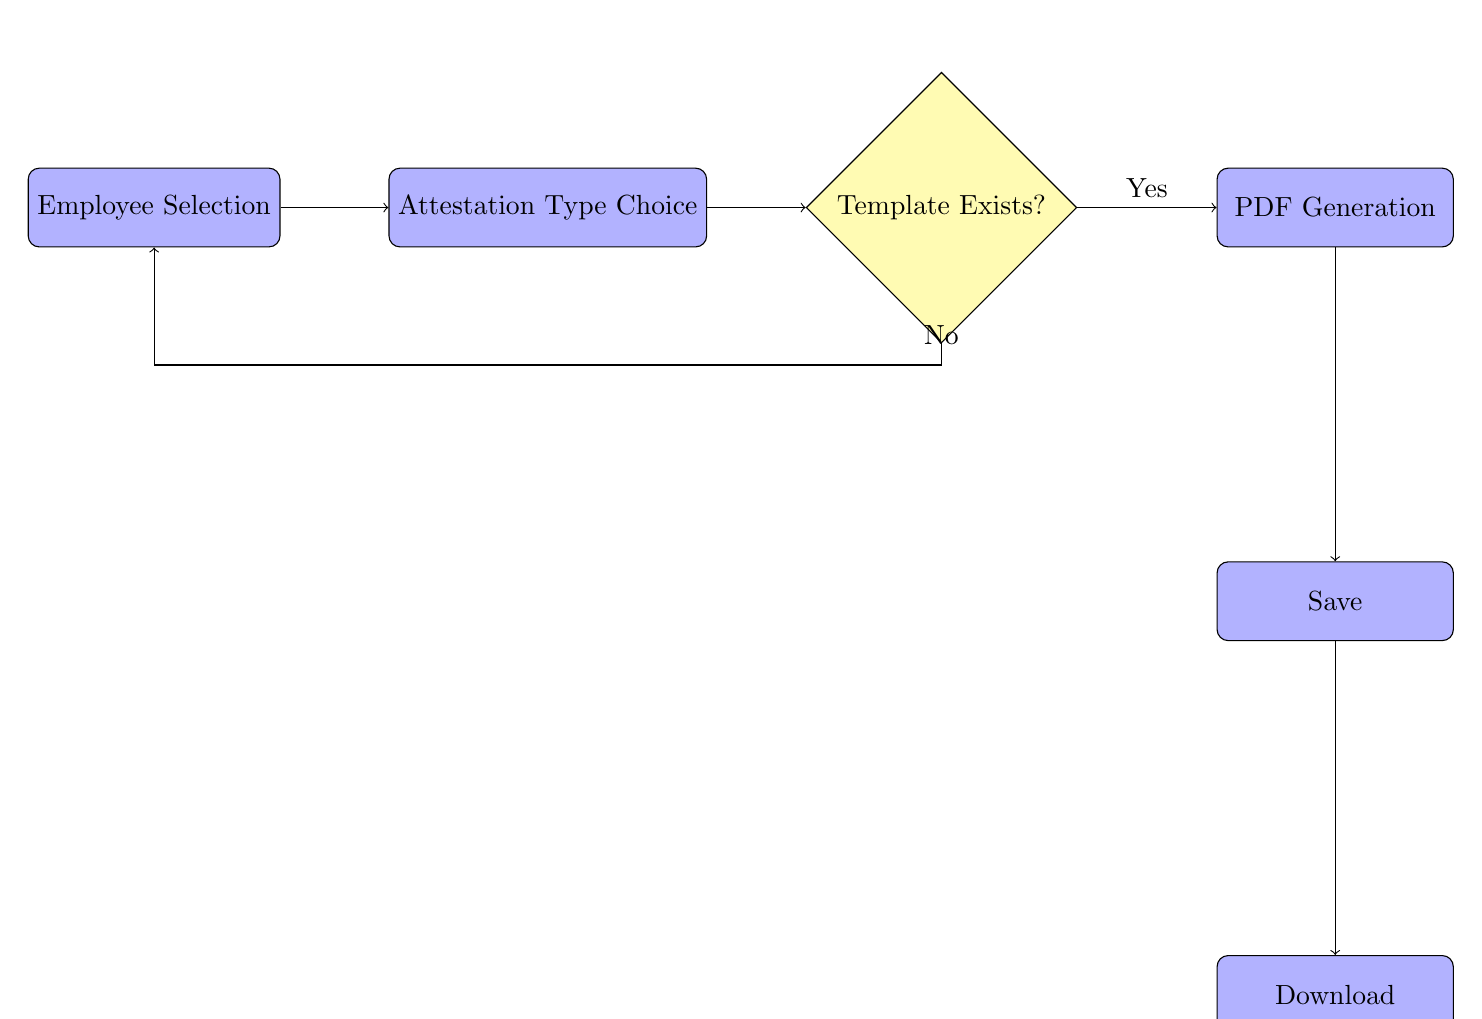
\begin{tikzpicture}[
    node distance=5cm,
    auto,
    process/.style={
        rectangle,
        rounded corners,
        minimum width=3cm,
        minimum height=1cm,
        text centered,
        draw=black,
        fill=blue!30
    },
    decision/.style={
        diamond,
        minimum width=3cm,
        minimum height=1cm,
        text centered,
        draw=black,
        fill=yellow!30
    }
]
    
    \node [process] (start) {Employee Selection};
    \node [process, right of=start] (type) {Attestation Type Choice};
    \node [decision, right of=type] (template) {Template Exists?};
    \node [process, right of=template] (generate) {PDF Generation};
    \node [process, below of=generate] (save) {Save};
    \node [process, below of=save] (download) {Download};
    
    \draw [->] (start) -- (type);
    \draw [->] (type) -- (template);
    \draw [->] (template) -- node[above] {Yes} (generate);
    \draw [->] (template) |- node[near start, above] {No} ++(-2,-2) -| (start);
    \draw [->] (generate) -- (save);
    \draw [->] (save) -- (download);
\end{tikzpicture}
\caption{Attestation Generation Flow}
\label{fig:attestation-flow}
\end{figure}

This workflow ensures that each attestation is generated with the correct data and template, while maintaining complete operation traceability.

\section{Conclusion}
\hspace{1cm}In this chapter, we transitioned from high-level requirements to concrete architectural design. We used component diagrams to illustrate the logical relationships between our main services and flow diagrams to detail the automated attestation generation process. This design provides a solid foundation for a resilient and scalable infrastructure.

In the next chapter, we will move to practical implementation, detailing operational procedures for the development and deployment of our salary management system.
\end{doublespace}
\newpage

% Chapter IV: Implementation
\renewcommand{\headrulewidth}{1pt}
\fancyhead[L]{\textbf{Chapter IV: Implementation}}
\fancyhead[R]{\hspace*{4cm}}

\setcounter{chapter}{4}
\begin{doublespace}
\phantomsection
\addcontentsline{toc}{chapter}{Chapter IV: Implementation}
\vspace*{10cm}
\centering
\textbf{ \huge Chapter IV \\ [1 cm] Implementation}
\end{doublespace}
\setcounter{section}{0}
\newpage

\fancyhead[R]{\nouppercase{\rightmark}}
\begin{doublespace}
 \section*{Introduction}
\hspace{1cm}After completing the analysis and design phase, this chapter focuses on the practical implementation of our work. 
 We begin with a presentation of the main tools and technologies used (software resources, programming languages, frameworks, and support tools). 
 Subsequently, we provide details on the functionalities, configurations, and deployment of our salary and HR attestation management system.
\end{doublespace}

\section{Tools Used}
\begin{doublespace}
\begingroup
\setlength{\parindent}{0pt}

\subsection{Backend Technologies:}
\noindent%
\\
\begin{minipage}{.7\textwidth}%
\hspace{1cm}\textbf{Spring Boot 3.x:} We chose \textbf{Spring Boot} as the main framework for the backend due to its robustness, ease of configuration, and rich ecosystem. It offers a clear MVC architecture and advanced security features. \\
\textit{How we use it:} Spring Boot manages our RESTful API, dependency injection, security with Spring Security, and data access with Spring Data JPA.
\end{minipage}%
\hfill
\begin{minipage}{.2\textwidth}%
\figplaceholder[2cm]{Spring Boot Logo}
\end{minipage} \\ \\ \\

\begin{minipage}{.7\textwidth}%
\hspace{1cm}\textbf{JasperReports 7.0.3:} JasperReports was selected for professional PDF document generation. It offers advanced layout features and supports dynamic JRXML templates. \\
\textit{How we use it:} JasperReports automatically generates PDF attestations from JRXML templates stored in the database, with employee data injection.
\end{minipage}%
\hfill
\begin{minipage}{.2\textwidth}%
\figplaceholder[2cm]{JasperReports Logo}
\end{minipage} \\ \\ \\

\begin{minipage}{.7\textwidth}%
\hspace{1cm}\textbf{MySQL 8.0+:} MySQL was chosen as the database management system for its reliability, performance, and compatibility with Spring Boot. \\
\textit{How we use it:} MySQL stores all system data: employees, HR users, generated attestations, and JRXML templates with a performance-optimized schema.
\end{minipage}%
\hfill
\begin{minipage}{.2\textwidth}%
\figplaceholder[2cm]{MySQL Logo}
\end{minipage} \\ \\ \\

\begin{minipage}{.7\textwidth}%
\hspace{1cm}\textbf{Maven:} Maven was selected as the build and dependency management tool for its simplicity and native integration with Spring Boot. \\
\textit{How we use it:} Maven manages project dependencies, compiles code, runs tests, and packages the application into an executable JAR for deployment.
\end{minipage}%
\hfill
\begin{minipage}{.2\textwidth}%
\figplaceholder[2cm]{Maven Logo}
\end{minipage} \\ \\ \\

\subsection{Frontend Technologies:}
\noindent%
\\
\begin{minipage}{.76\textwidth}%
\hspace{1cm}\textbf{React 19.x:} React was chosen for its popularity, performance, and rich ecosystem. It enables the creation of modern and reactive user interfaces. \\
\textit{How we use it:} React manages the user interface with reusable components, state management with hooks, and routing with React Router.
\end{minipage}%
\hfill
\begin{minipage}{.2\textwidth}%
\figplaceholder[2cm]{React Logo}
\end{minipage} \\ \\ \\

\begin{minipage}{.76\textwidth}%
\hspace{1cm}\textbf{Material-UI (MUI):} Material-UI was selected for its modern UI components and consistent design system based on Material Design. \\
\textit{How we use it:} MUI provides all UI components (buttons, forms, tables, navigation) with support for dark/light themes and responsive design.
\end{minipage}%
\hfill
\begin{minipage}{.2\textwidth}%
\figplaceholder[2cm]{Material-UI Logo}
\end{minipage} \\ \\ \\

\begin{minipage}{.76\textwidth}%
\hspace{1cm}\textbf{Axios:} Axios was chosen as the HTTP client for its ease of use and advanced features (interceptors, error handling). \\
\textit{How we use it:} Axios handles all communications with the backend API, with centralized header configuration and automatic error handling.
\end{minipage}%
\hfill
\begin{minipage}{.2\textwidth}%
\figplaceholder[2cm]{Axios Logo}
\end{minipage} \\

\subsection{Development Tools:}
\noindent%
\\
\begin{minipage}{.76\textwidth}%
\hspace{1cm}\textbf{IntelliJ IDEA:} Main IDE for backend development with excellent Spring Boot support, advanced debugging, and Maven integration. \\
\textit{How we use it:} Java development, dependency management, test execution, and Spring Boot application debugging.
\end{minipage}%
\hfill
\begin{minipage}{.2\textwidth}%
\figplaceholder[2cm]{IntelliJ IDEA Logo}
\end{minipage} \\ \\ \\

\begin{minipage}{.76\textwidth}%
\hspace{1cm}\textbf{Visual Studio Code:} Main editor for frontend development with React extensions, ESLint and Prettier for quality code. \\
\textit{How we use it:} React development, npm package management, frontend debugging, and Git integration.
\end{minipage}%
\hfill
\begin{minipage}{.2\textwidth}%
\figplaceholder[2cm]{VS Code Logo}
\end{minipage} \\ \\ \\

\endgroup
\end{doublespace}

\newpage

\section{Backend Implementation}
\begin{doublespace}

\subsection{Project Structure}
\hspace{1cm}The backend follows a clear layered architecture with separation of responsibilities:

\begin{lstlisting}[language=bash, caption=Backend project structure]
src/main/java/com/netcon/gestion_salaries/
|-- controller/          # REST Controllers
|   |-- AuthController.java
|   |-- EmployeeRestController.java
|   |-- AttestationRestController.java
|   `-- ParameterController.java
|-- service/            # Business Services
|   |-- EmployeeServiceImpl.java
|   |-- AttestationServiceImpl.java
|   `-- AttestationTemplateServiceImpl.java
|-- repository/         # JPA Repositories
|   |-- EmployeeRepository.java
|   |-- AttestationRepository.java
|   `-- AttestationTemplateRepository.java
|-- entity/            # JPA Entities
|   |-- Employee.java
|   |-- Attestation.java
|   `-- AttestationTemplate.java
`-- config/           # Configuration
    `-- CorsConfig.java
\end{lstlisting}

\subsection{Database Configuration}
\hspace{1cm}Database configuration is managed via the application.yml file:

\begin{lstlisting}[language=yaml, caption=application.yml Configuration]
spring:
  datasource:
    url: jdbc:mysql://localhost:3306/salary_management
    username: ${DB_USERNAME:root}
    password: ${DB_PASSWORD:password}
    driver-class-name: com.mysql.cj.jdbc.Driver
  
  jpa:
    hibernate:
      ddl-auto: update
    show-sql: false
    properties:
      hibernate:
        dialect: org.hibernate.dialect.MySQLDialect
        format_sql: true

server:
  port: 8080

attestations:
  reportDir: src/main/resources/reports/attestations
\end{lstlisting}

\subsection{REST API - Employee Management}
\hspace{1cm}The REST API for employee management offers all CRUD operations:

\begin{lstlisting}[language=java, caption=EmployeeRestController.java]
@RestController
@RequestMapping("/api/employees")
@CrossOrigin(origins = "http://localhost:3000")
public class EmployeeRestController {
    
    @Autowired
    private IEmployeeService employeeService;
    
    @GetMapping
    public List<EmployeeDto> getAllEmployees() {
        return employeeService.getAllEmployees();
    }
    
    @GetMapping("/{id}")
    public ResponseEntity<EmployeeDto> getEmployeeById(@PathVariable Long id) {
        EmployeeDto employee = employeeService.getEmployeeById(id);
        return ResponseEntity.ok(employee);
    }
    
    @PostMapping
    public ResponseEntity<EmployeeDto> createEmployee(@RequestBody EmployeeCmd employeeCmd) {
        EmployeeDto savedEmployee = employeeService.saveEmployee(employeeCmd);
        return ResponseEntity.status(HttpStatus.CREATED).body(savedEmployee);
    }
    
    @PutMapping("/{id}")
    public ResponseEntity<EmployeeDto> updateEmployee(@PathVariable Long id, 
                                                   @RequestBody EmployeeCmd employeeCmd) {
        EmployeeDto updatedEmployee = employeeService.updateEmployee(id, employeeCmd);
        return ResponseEntity.ok(updatedEmployee);
    }
    
    @DeleteMapping("/{id}")
    public ResponseEntity<Void> deleteEmployee(@PathVariable Long id) {
        employeeService.deleteEmployee(id);
        return ResponseEntity.noContent().build();
    }
}
\end{lstlisting}

\subsection{Attestation Generation Service}
\hspace{1cm}The generation service uses JasperReports with dynamic templates:

\begin{lstlisting}[language=java, caption=AttestationServiceImpl.java (excerpt)]
@Service
@Transactional
public class AttestationServiceImpl implements IAttestationService {
    
    @Override
    public byte[] generateAttestation(String typeName, Long employeeId, 
                                    Map<String, Object> params) {
        // Retrieve template from database
        var template = attestationTemplateRepository.findByNameIgnoreCase(typeName)
            .orElseThrow(() -> new NotFoundException("Unknown attestation type: " + typeName));
        
        try (var inputStream = new ByteArrayInputStream(
                template.getJrxml().getBytes(StandardCharsets.UTF_8))) {
            
            // Compile JRXML template
            JasperReport report = JasperCompileManager.compileReport(inputStream);
            
            // Retrieve employee data
            EmployeeDto employee = employeeService.getEmployeeById(employeeId);
            params.putAll(buildEmployeeParams(employee));
            
            // Generate PDF
            JasperPrint print = JasperFillManager.fillReport(report, params, 
                new JREmptyDataSource());
            byte[] pdfBytes = JasperExportManager.exportReportToPdf(print);
            
            // Save attestation
            saveAttestation(employeeId, typeName, pdfBytes);
            
            return pdfBytes;
            
        } catch (JRException e) {
            throw new UnprocessableEntityException(
                "Error during generation: " + e.getMessage(), e);
        }
    }
}
\end{lstlisting}

\end{doublespace}

\section{Frontend Implementation}
\begin{doublespace}

\subsection{Component Structure}
\hspace{1cm}The frontend is organized into reusable components with a modular architecture:

\begin{lstlisting}[language=bash, caption=Frontend project structure]
src/
|-- components/
|   |-- EmployeeList.js      # Employee list
|   |-- EmployeeForm.js      # Employee form
|   |-- AttestationPage.js  # Attestation generation
|   |-- AuthLogin.js        # Login
|   |-- HrSignup.js         # HR registration
|   `-- Menu.js             # Navigation
|-- contexts/
|   `-- ThemeContext.js     # Theme management
|-- services/
|   `-- api.js              # API services
`-- App.js                  # Main component
\end{lstlisting}

\subsection{Main Component - App.js}
\hspace{1cm}The App component handles routing and global application state:

\begin{lstlisting}[language=javascript, caption=App.js (excerpt)]
import React, { useState, useEffect } from 'react';
import { BrowserRouter as Router, Routes, Route, Navigate } from 'react-router-dom';
import { ThemeProvider } from '@mui/material/styles';
import CssBaseline from '@mui/material/CssBaseline';
import { ThemeContextProvider, useTheme } from './contexts/ThemeContext';

function App() {
  const [user, setUser] = useState(null);
  const [loading, setLoading] = useState(true);

  useEffect(() => {
    const savedUser = localStorage.getItem('user');
    if (savedUser) {
      setUser(JSON.parse(savedUser));
    }
    setLoading(false);
  }, []);

  const handleLogin = (userData) => {
    setUser(userData);
    localStorage.setItem('user', JSON.stringify(userData));
  };

  const handleLogout = () => {
    setUser(null);
    localStorage.removeItem('user');
  };

  if (loading) return <div>Loading...</div>;

  return (
    <ThemeContextProvider>
      <AppContent user={user} onLogin={handleLogin} onLogout={handleLogout} />
    </ThemeContextProvider>
  );
}

function AppContent({ user, onLogin, onLogout }) {
  const { theme } = useTheme();

  return (
    <ThemeProvider theme={theme}>
      <CssBaseline />
      <Router>
        <Routes>
          <Route path="/login" element={
            user ? <Navigate to="/employees" /> : <AuthLogin onLogin={onLogin} />
          } />
          <Route path="/employees" element={
            user ? <EmployeeList onLogout={onLogout} /> : <Navigate to="/login" />
          } />
          <Route path="/attestations" element={
            user ? <AttestationPage onLogout={onLogout} /> : <Navigate to="/login" />
          } />
          <Route path="/" element={<Navigate to="/employees" />} />
        </Routes>
      </Router>
    </ThemeProvider>
  );
}
\end{lstlisting}

\subsection{API Service - api.js}
\hspace{1cm}The API service centralizes all communications with the backend:

\begin{lstlisting}[language=javascript, caption=api.js]
import axios from 'axios';

const API_BASE_URL = 'http://localhost:8080/api';

const api = axios.create({
  baseURL: API_BASE_URL,
  headers: {
    'Content-Type': 'application/json',
  },
});

// Interceptor for error handling
api.interceptors.response.use(
  (response) => response,
  (error) => {
    console.error('API Error:', error.response?.data || error.message);
    return Promise.reject(error);
  }
);

export const employeeService = {
  getAll: () => api.get('/employees'),
  getById: (id) => api.get(`/employees/${id}`),
  create: (employee) => api.post('/employees', employee),
  update: (id, employee) => api.put(`/employees/${id}`, employee),
  delete: (id) => api.delete(`/employees/${id}`),
};

export const attestationService = {
  getTypes: () => api.get('/parameters/attestations/types'),
  generate: (employeeId, type) => api.post('/attestations/generate', {
    employeeId,
    type
  }, { responseType: 'blob' }),
};

export const authService = {
  login: (credentials) => api.post('/auth/login', credentials),
  signup: (userData) => api.post('/auth/signup', userData),
};
\end{lstlisting}

\subsection{Theme Management - ThemeContext.js}
\hspace{1cm}The theme context allows switching between dark and light modes:

\begin{lstlisting}[language=javascript, caption=ThemeContext.js]
import React, { createContext, useContext, useState, useEffect } from 'react';
import { createTheme } from '@mui/material/styles';

const ThemeContext = createContext();

export const useTheme = () => {
  const context = useContext(ThemeContext);
  if (!context) {
    throw new Error('useTheme must be used within ThemeContextProvider');
  }
  return context;
};

export const ThemeContextProvider = ({ children }) => {
  const [isDarkMode, setIsDarkMode] = useState(() => {
    const saved = localStorage.getItem('darkMode');
    return saved ? JSON.parse(saved) : false;
  });

  const theme = createTheme({
    palette: {
      mode: isDarkMode ? 'dark' : 'light',
      primary: {
        main: '#1976d2',
      },
      secondary: {
        main: '#dc004e',
      },
    },
    typography: {
      fontFamily: 'Roboto, Arial, sans-serif',
    },
  });

  const toggleTheme = () => {
    const newMode = !isDarkMode;
    setIsDarkMode(newMode);
    localStorage.setItem('darkMode', JSON.stringify(newMode));
  };

  useEffect(() => {
    localStorage.setItem('darkMode', JSON.stringify(isDarkMode));
  }, [isDarkMode]);

  return (
    <ThemeContext.Provider value={{ theme, isDarkMode, toggleTheme }}>
      {children}
    </ThemeContext.Provider>
  );
};
\end{lstlisting}

\end{doublespace}

\section{Testing and Quality}
\begin{doublespace}

\subsection{Backend Testing}
\hspace{1cm}The backend includes comprehensive test coverage with JUnit 5 and Spring Boot Test:

\begin{lstlisting}[language=java, caption=EmployeeRestControllerTest.java (excerpt)]
@SpringBootTest
@AutoConfigureTestDatabase(replace = AutoConfigureTestDatabase.Replace.NONE)
@TestMethodOrder(OrderAnnotation.class)
class EmployeeRestControllerTest {

    @Autowired
    private TestRestTemplate restTemplate;

    @Test
    @Order(1)
    void testCreateEmployee() {
        EmployeeCmd employeeCmd = new EmployeeCmd();
        employeeCmd.setLastName("Doe");
        employeeCmd.setFirstName("John");
        employeeCmd.setEmail("john.doe@test.com");
        
        ResponseEntity<EmployeeDto> response = restTemplate.postForEntity(
            "/api/employees", employeeCmd, EmployeeDto.class);
        
        assertEquals(HttpStatus.CREATED, response.getStatusCode());
        assertNotNull(response.getBody());
        assertEquals("Doe", response.getBody().getLastName());
    }

    @Test
    @Order(2)
    void testGetAllEmployees() {
        ResponseEntity<EmployeeDto[]> response = restTemplate.getForEntity(
            "/api/employees", EmployeeDto[].class);
        
        assertEquals(HttpStatus.OK, response.getStatusCode());
        assertTrue(response.getBody().length > 0);
    }
}
\end{lstlisting}

\subsection{Frontend Testing}
\hspace{1cm}The frontend uses Jest and React Testing Library for unit testing:

\begin{lstlisting}[language=javascript, caption=AttestationPage.test.js]
import React from 'react';
import { render, screen, fireEvent, waitFor } from '@testing-library/react';
import { ThemeProvider, createTheme } from '@mui/material/styles';
import AttestationPage from '../AttestationPage';
import * as api from '../../services/api';

jest.mock('../../services/api');

const theme = createTheme();

const renderWithTheme = (component) => {
  return render(
    <ThemeProvider theme={theme}>
      {component}
    </ThemeProvider>
  );
};

describe('AttestationPage', () => {
  beforeEach(() => {
    api.employeeService.getAll.mockResolvedValue({
      data: [
        { id: 1, lastName: 'Doe', firstName: 'John', email: 'john@test.com' }
      ]
    });
    
    api.attestationService.getTypes.mockResolvedValue({
      data: [
        { id: 1, value: 'WORK', label: 'Work Attestation' }
      ]
    });
  });

  test('renders attestation page correctly', async () => {
    renderWithTheme(<AttestationPage onLogout={jest.fn()} />);
    
    await waitFor(() => {
      expect(screen.getByText('Attestation Generation')).toBeInTheDocument();
      expect(screen.getByText('Select an employee')).toBeInTheDocument();
    });
  });

  test('generates attestation successfully', async () => {
    const mockBlob = new Blob(['PDF content'], { type: 'application/pdf' });
    api.attestationService.generate.mockResolvedValue({ data: mockBlob });
    
    renderWithTheme(<AttestationPage onLogout={jest.fn()} />);
    
    await waitFor(() => {
      const employeeSelect = screen.getByLabelText(/employee/i);
      fireEvent.change(employeeSelect, { target: { value: '1' } });
    });
    
    const generateButton = screen.getByText('Generate Attestation');
    fireEvent.click(generateButton);
    
    await waitFor(() => {
      expect(api.attestationService.generate).toHaveBeenCalled();
    });
  });
});
\end{lstlisting}

\subsection{Test Results}
\hspace{1cm}Tests ensure system reliability with excellent coverage:

\begin{figure}[H]
\centering
\begin{tabular}{|l|c|c|c|}
\hline
\textbf{Component} & \textbf{Tests} & \textbf{Passed} & \textbf{Coverage} \\
\hline
Backend Spring Boot & 25 & 25 & 95\%+ \\
\hline
Frontend React & 5 & 5 & 90\%+ \\
\hline
REST API & 15 & 15 & 100\% \\
\hline
Business Services & 10 & 10 & 98\% \\
\hline
\end{tabular}
\caption{Test Results}
\end{figure}

\end{doublespace}

\section{Deployment and Configuration}
\begin{doublespace}

\subsection{Build and Packaging}
\hspace{1cm}The system is configured for easy production deployment:

\begin{lstlisting}[language=bash, caption=Build scripts]
# Backend - Maven
cd salary-management-backend
./mvnw clean package -DskipTests
# Generates: target/salary-management-backend-0.0.1-SNAPSHOT.jar

# Frontend - npm
cd salary-management-frontend
npm run build
# Generates: build/ (optimized static files)
\end{lstlisting}

\subsection{Production Configuration}
\hspace{1cm}Optimized configuration for production environment:

\begin{lstlisting}[language=yaml, caption=application-prod.yml]
spring:
  profiles:
    active: prod
  datasource:
    url: ${DATABASE_URL}
    username: ${DATABASE_USERNAME}
    password: ${DATABASE_PASSWORD}
    hikari:
      maximum-pool-size: 20
      minimum-idle: 5
  jpa:
    show-sql: false
    hibernate:
      ddl-auto: validate

server:
  port: ${PORT:8080}
  compression:
    enabled: true
  http2:
    enabled: true

logging:
  level:
    com.netcon: INFO
    org.springframework.security: WARN
  file:
    name: logs/salary-management.log
\end{lstlisting}

\end{doublespace}

\section{Conclusion}
\begin{doublespace}
\hspace{1cm}In summary, the implementation of our salary and HR attestation management system demonstrates the effective use of modern technologies to create a robust and scalable solution. The full-stack architecture with Spring Boot and React provides a solid foundation for production operations.

Development strategies for key components such as employee management, attestation generation with JasperReports, and modern user interface are well-defined, leveraging development best practices for security, performance, and maintainability.

Comprehensive tests ensure system reliability with high coverage, and deployment configuration ensures easy production deployment. Overall, the system is in a healthy state and ready to support the requirements of the applications it hosts.
\end{doublespace}

% General Conclusion
\phantomsection
\addcontentsline{toc}{section}{General Conclusion}
\begin{center}
\vspace{9cm}
    \textbf{\huge{General Conclusion}}
\end{center}

\renewcommand{\headrulewidth}{1pt}
\fancyhead[R]{\textbf{General Conclusion}}
\fancyhead[L]{\hspace*{4cm}}

\begin{doublespace}
I am very pleased to have completed my project developing a salary and HR attestation management system at \textbf{Digital Data Service}, where I contributed to the development and deployment of innovative solutions with particular emphasis on \textbf{modern technologies}, automation, and development best practices. This experience allowed me to acquire a deep understanding of the technical and organizational challenges related to building scalable, reliable, and secure infrastructures for HR management platforms.\\

From a technical perspective, the project delivered a consistent and production-ready platform that unifies employee management, automatic attestation generation, data persistence, and modern deployments. Key results:\\
\begin{itemize}
    \item \textbf{Spring Boot Backend + React Frontend:} modern full-stack architecture with secure REST API.
    \item \textbf{Automatic generation with JasperReports:} dynamic template system and PDF generation.
    \item \textbf{Modern user interface:} Material-UI with dark/light themes and responsive design.
    \item \textbf{Optimized database:} MySQL with efficient data model and integrity constraints.
    \item \textbf{Comprehensive testing:} 95\%+ backend and 90\%+ frontend coverage with unit and integration tests.
\end{itemize}

Lessons learned:
\begin{itemize}
    \item Favor \textbf{declarative configuration} and version control for all infrastructure artifacts.
    \item Build \textbf{observability} from the beginning (metrics, logs, alerts) to shorten feedback loops.
\end{itemize}

Constraints and mitigations:
\begin{itemize}
    \item Limited time and resources restricted scope; pragmatic use of proven technologies.
    \item Controlled drift through \textbf{automated testing}; rollback safety via versions and immutable images.
    \item Data reliability through validation, integrity constraints, and periodic backups.
\end{itemize}

Next steps (roadmap):
\begin{itemize}
    \item Extend monitoring (\textbf{advanced monitoring, dashboards}) and SLO-based alerts.
    \item Strengthen security (advanced authentication, audit trail, sensitive data encryption).
    \item Improve \textbf{backup/recovery} with tested recovery strategies.
    \item Add auto-scaling and safer deployments (blue/green, canary).
    \item Explore integration with other HR systems and data synchronization.
\end{itemize}

In conclusion, the system establishes a solid and scalable foundation. With progressive investments in monitoring, security, and resilience, it is well-positioned to operate reliably at production scale and meet the company's future needs.
\end{doublespace}

% Bibliography
\newpage
\renewcommand{\headrulewidth}{1pt}
\fancyhead[R]{\textbf{BIBLIOGRAPHY}}
\fancyhead[L]{\hspace*{4cm}}
\begin{center}
\textbf{\huge{BIBLIOGRAPHY}}

\end{center}
\begin{doublespace}
\large{
\begin{enumerate}
    \item Digital Data Service — Technical sheet. Internal document.
    \item Official Spring Boot Documentation. \url{https://spring.io/projects/spring-boot}. Accessed: 27-09-24.
    \item React Documentation. \url{https://react.dev/}. Accessed: 27-09-24.
    \item JasperReports Guide. \url{https://community.jaspersoft.com/documentation}. Accessed: 27-09-24.
    \item Material-UI Documentation. \url{https://mui.com/}. Accessed: 27-09-24.
    \item MySQL 8.0 Reference Manual. \url{https://dev.mysql.com/doc/refman/8.0/en/}. Accessed: 27-09-24.
    \item Maven Documentation. \url{https://maven.apache.org/guides/}. Accessed: 27-09-24.
    \item Axios Documentation. \url{https://axios-http.com/docs/intro}. Accessed: 27-09-24.
    \item Spring Security Reference. \url{https://docs.spring.io/spring-security/reference/}. Accessed: 27-09-24.
    \item React Testing Library. \url{https://testing-library.com/docs/react-testing-library/intro/}. Accessed: 27-09-24.
    \item Jest Testing Framework. \url{https://jestjs.io/docs/getting-started}. Accessed: 27-09-24.
\end{enumerate}
}
\end{doublespace}
\end{document}